\documentclass[twosided,a4,10pt]{article}
\usepackage[utf8]{inputenc}
\usepackage{amsmath}
\usepackage{amsfonts}
\usepackage{amssymb}
\usepackage{textcomp}
\usepackage{german}
\usepackage{graphicx}
\usepackage[usenames,dvipsnames]{xcolor}
\usepackage{pifont}
\usepackage{nicefrac}
\usepackage{sectsty}

% ------
% Fonts and typesetting settings
\usepackage[sc]{mathpazo}
\usepackage[T1]{fontenc}
\linespread{1.1} % Palatino needs more space between lines
\usepackage{microtype}
\subsectionfont{\fontsize{10}{15}\selectfont}

% ------
% Page layout
\usepackage[hmarginratio=1:1,top=32mm,columnsep=20pt]{geometry}
\usepackage[font=it]{caption}
\usepackage{paralist}
\usepackage{multicol}

%------
%caption hack
\usepackage{caption}

\DeclareCaptionType{faltung}[][List of equations]
\captionsetup[faltung]{labelformat=empty}

% ------
% Abstract
\usepackage{abstract}
	\renewcommand{\abstractnamefont}{\normalfont\bfseries}
	\renewcommand{\abstracttextfont}{\normalfont\small\itshape}


% ------
% Titling (section/subsection)
\usepackage{titlesec}
%\renewcommand\thesection{\Roman{section}}
\titleformat{\section}[block]{\large\scshape\centering}{\thesection.}{1em}{}

% ------
% Clickable URLs (optional)
\usepackage[hyphens]{url}
\usepackage{hyperref}

% ------
% Header/footer
\usepackage{fancyhdr}
	\pagestyle{fancy}
%	\fancyhead{}
%	\fancyfoot[C]{WIS WS 2017/18 $\cdot$
%          Software Engineering $\cdot$ Prof. Dr. Dünnweber}
	\fancyhead[R]{OTH Regensburg $\cdot$ Fakultät IM}
%	\fancyfoot[RO,LE]{\thepage}
	\fancyfoot[L]{WIS $\cdot$ WS 2017/18}
	\fancyfoot[R]{Prof. Dr. Dünnweber}
	\fancyfoot[C]{\thepage}


% ------
% Maketitle metadata
\title{\vspace{-5mm}%
	\fontsize{20pt}{10pt}\selectfont
	\textbf{Inhaltsbasierte Musikempfehlung mit Convolutional Neuronalen Netzwerken}
	}	
\vspace{-5mm}\date{}
\author{
	\large\begin{minipage}[t]{0.5\linewidth}
		\begin{center}
			\textsc{Weidhas Philipp}\\[2mm]
			\normalsize	Matr.nr: 123456\\
			\normalsize
			\href{mailto:philipp.weidhas@st.oth-regensburg.de}
			{philipp.weidhas@st.oth-regensburg.de}      
		\end{center}
	\end{minipage}        
	\begin{minipage}[t]{0.5\linewidth}
         \begin{center}
           	\textsc{Wildgruber Markus}\\[2mm]
                 \normalsize	Matr.nr: 123456\\
                 \normalsize
                 \href{mailto:markus.wildgruber@stud.oth-regensburg.de}
                 {markus.wildgruber@stud.oth-regensburg.de}      
         \end{center}
       \end{minipage}
     }




%%%%%%%%%%%%%%%%%%%%%%%%
\begin{document}

\maketitle
\thispagestyle{fancy}

	

\begin{multicols}{2}

\begin{abstract}
\noindent Hier kommt die Zusammenfassung...
\end{abstract}


\section{Einleitung}
Im ersten Halbjahr des Jahres 2017 wurden 62\% der Einnahmen der amerikanischen Musikindustrie durch Streaming Plattformen (wie Spotify, Apple Music, Pandora etc.) erzielt. Im Vergleich zu Vorjahr erhöhten sich dadurch die Einnahmen um 48\% auf 2.5\$ Milliarde \cite{friedlander}\cite{rys}. Es zeigt sich, dass automatisierte Empfehlungssysteme weit verbreitet sind.\newline
Obwohl diese in den letzten Jahren viel erforscht wurden, existieren noch Probleme, die bislang zu wenig in Musikempfehlungssystemen berücksichtigt wurden. Neben der große Anzahl an verschiedenen Stile und Genres, beeinflussen sowohl soziales- und geographisches Umfeld, sowie der aktuelle Gemütszustandes die Vorliebe eines Hörers. \cite{oord}\newline\\
Nach Schedl \cite{schedl} gibt es in der Musik Information Retrieval (MIR) vier Kategorien die einen Einfluß auf die Wahrnehmung von ähnlicher Musik haben. \textit{Musikinhalt} bezieht sich auf alles, dass aus dem Signal selbst herausgefiltert werden kann. Dazu zählen Aspekte wie der Rhythmus, die Melodie, die Harmonie oder die Stimmung eines Stücks.\cite{knees}\newline
Als \textit{Musikkontext} versteht man alle Aspekte, die nicht aus dem Audiosignal abgeleitet werden, sondern Informationen die über ein Musikstück bekannt sind. Beispielsweise Metadaten wie der Titel eines Lieds, das Genre, Name des Künstlers oder das Erscheinungsjahr \cite{knees}.\newline
Die \textit{Benutzereigenschaften} beziehen sie auf Persönlichkeitsmerkmale, wie Geschmack, musikalisches Wissen und Erfahrung oder den demographischen Hintergrund \cite{knees}.\newline
Im Unterschied dazu steht der \textit{Benutzerkontext}, der sich auf die aktuelle Situation des Hörers bezieht. Dabei wird er durch seine Umgebung, seiner Stimmung oder der aktuellen Aktivität beeinflußt \cite{knees}.\newline
Bislang werden Informationen über den Hörer durch ein Benutzerprofil repräsentiert. Das Profil enthält oftmals nur wenig Hintergrund Informationen des Hörers und beschränkt sich auf Lieder, die ein Benutzer angehört und bewertet hat \cite{oord}. Das Nutzen dieser Daten um Musikvorschläge zu machen wird als Kollaboratives Filtern (CF) bezeichnet. In der Studie von Vigliensoni und Fujinaga \cite{vigliensoni} zeigt sich ein deutlicher Unterschied zwischen herkömmlichen Benutzerprofilen und das Einfügen von Zusatzinformationen. Durch das Hinzufügen der Features demographischen Hintergrund und Entdeckergeist des Hörers konnte im Vergleich zu einem herkömmlichen Profil eine 12\% besser Genauigkeit erreicht werden.\newline\\
Der weitere Verlauf der wissenschaftlichen Arbeit ist wie folgt organisiert. Im 2. Abschnitt werden verschieden Ansätze in den jeweiligen Methodenbereichen vorgestellt. Im 3. Kapitel werden die erfolgreichsten Ansätze miteinander verglichen. Teil 4 zeigt ein eigenes Experiment zu dem Thema. Abschnitt 5 schließt diese Arbeit ab und diskutiert zukünftige Forschungsrichtungen. //TO DO

\section{Methoden zur Musikempfehlung}
Es gibt vier verschiedene Methoden, die in Musikempfehlungssystemen verwendet werden: kollaboratives -, inhaltsbasierte -, kontext-basiertes Filtern und die hybride Methode \cite{kaitila}.

Zur Lösung des in der Einleitung erläuterten Problems, gibt es bereits mehrere erprobte und in verschiedenster Weise angewandte Problemlösungsansätze. Diese Ansätze werden in diesem Kapitel nun eingehend erläutert. Im genauen werden aktuell 3 verschiedene Verfahren angewandt, diese sind ein inhaltsbezogener Ansatz, ein Kontextbasierenender Ansatz und ein Hybrides Verfahren das beide Verfahren in sich vereint.

\subsection{Kollaborativer Filtern}
Kollaboratives Filtern prognostiziert Vorlieben eines Hörers, indem es aus unterschiedlichen Benutzer-Lied Verhältnissen lernt. Es basiert auf der Annahme, dass Verhalten und Bewertungen andere Nutzer auf eine vernünftige Vorhersage für den aktiven Benutzer schließen lassen \cite{celma}. Durch explizite oder implizite Rückmeldung an das Empfehlungssystem empfiehlt dieses neue Lieder, indem es Gemeinsamkeiten auf Basis der Bewertungen vergleicht \cite{mcfee}.\newline
Eine Vorhersage, ob ein Lied einem Benutzer vorgeschlagen werden soll, kann auf zwei verschiedene Arten erfolgen. In der ersten Methode werden Ähnlichkeiten von Bewertungsmustern verglichen. Lieder werden als ähnlich erachtet, wenn sie von denselben Benutzern positiv bewertet wurden. Die zweite Methode berechnet ihre Vorhersage in dem sie ähnliche Profile zu einem Bestimmten sucht und deren Positiv bewerteten Lieder als Vorschlag benutzt. \cite{ekstrandand}\newline
Verschiedene Studien (\cite{mcfee}\cite{barrington}) zeigen das CF alternative Methoden in der Genauigkeit übertrifft, weshalb es nicht nur im Bereich der Musikempfehlung als die Erfolgreichste gilt.\newline
Trotz der Popularität des CF gibt Probleme die bei der Verwendung der Methode beachtet werden müssen. Beim Cold-Start Problem liegen noch keine Bewertungen für ein Lied vor, wodurch es auch nicht vorgeschlagen werden kann. Dasselbe Problem gibt es bei einem neuen Benutzer, diesem kann kein guter Vorschlag gemacht werden, da es an Information mangelt welche Art von Musik ihm gefällt. \cite{celma} Neben dem Cold-Start Problem gibt es noch weitere Probleme die in \cite{celma} aufgeführt werden.

\subsection{Inhaltsbasierter Filter}
TODO: Inhaltsbasierend, Inhaltsbezogen ist meiner Meinung nach der Falsche ausdruck dafür! :TODO
Als erstes wird nun ein genauerer Blick auf den inhaltsbezogenen Ansatz geworfen. Mittels diesem Verfahrens werden Nutze Musikstücke aufgrund aus Lieder gewonnener Informationen vorgeschlagen. Dies bedeutet im Detail dass aus den Musikstücken mittels verschiedenster Metriken die Audio Signale eines Liedes analysiert werden um Erkenntnisse über die Stimmung eines Liedes, die Frequenz oder Rythmus zu erhalten. Auf Grund dieser Informationen können Stücke dem Konsumenten vorgeschlagen werden die einen gleichen oder sehr ähnlichen Inhalt bieten.

\subsection{Kontextbasierter Filter}
Das zweite Verfahren welches nun eingehender betrachtet wird, ist ein kontextbasiertes Verfahren. Im diesen Verfahren wird der Ansatz verfolgt das Lieder einem Nutzer auf Grundlage von Nutzungsverhalten anderer Anwender der gleichen Plattform vorgeschlagen werden. In der Praktischen Umsetzung bedeutet dies, hört ein Anwender ein bestimmtes Musikstück wird im vom System, Lieder vorgeschlagen welche Nutzer in Zeitraum davor nach diesem diesem Stück hörten. Dieses Verfahren geht davon aus das durch die Verbindung der Lieder durch vorhergehende Aufrufe eine gute Aussage darüber getroffen werden kann wie gut diese Stücke zusammen passen. Werden Lieder häufig Nacheinander gehört, wird diese Verbindung höher bewertet und die Empfehlung häufiger ausgesprochen. Auch wird das Verhalten und der Musikgeschmack des Kunden selbst analysiert um so über Ähnlichkeiten der Kundenpräferenzen mit derer anderer, diesen wiederum bessere Empfehlungen aussprechen zu können. So werden Lieder einem Musikstil zugeordnet und so zielgerichtet dem Nutzer nahegelegt.

\subsection{Kontext-basierter Filter}
Das zweite Verfahren welches nun eingehender betrachtet wird, ist ein kontextbasiertes Verfahren. Im diesen Verfahren wird der Ansatz verfolgt das Lieder einem Nutzer auf Grundlage von Nutzungsverhalten anderer Anwender der gleichen Plattform vorgeschlagen werden. In der Praktischen Umsetzung bedeutet dies, hört ein Anwender ein bestimmtes Musikstück wird im vom System, Lieder vorgeschlagen welche Nutzer in Zeitraum davor nach diesem diesem Stück hörten. Dieses Verfahren geht davon aus das durch die Verbindung der Lieder durch vorhergehende Aufrufe eine gute Aussage darüber getroffen werden kann wie gut diese Stücke zusammen passen. Werden Lieder häufig Nacheinander gehört, wird diese Verbindung höher bewertet und die Empfehlung häufiger ausgesprochen. Auch wird das Verhalten und der Musikgeschmack des Kunden selbst analysiert um so über Ähnlichkeiten der Kundenpräferenzen mit derer anderer, diesen wiederum bessere Empfehlungen aussprechen zu können. So werden Lieder einem Musikstil zugeordnet und so zielgerichtet dem Nutzer nahegelegt.

\subsection{Hybride Methode}
Bei hybriden Methoden werden verschiedene Filtertechniken mit einer verbunden, wodurch ein besseres Vorschlagergebnis erzielt wird. Meistens wird ein kollaborativer Filter mit einem anderem kombiniert. Durch diese Kombination können Nachteile einer einzelnen Methode verschwinden. \cite{burke}\newline
Burke \cite{burke} definiert unterschiedliche Arten von Hybrid-Filtern, die von verschiedenen Forschern benutzt wurden.\newline
Als \textit{gewichtet} wird eine hybride Methode bezeichnet, die alle Ergebnisse einzelner Empfehlungen zusammenfügt und daraus den Wert des empfohlenen Liedes errechnet. Durch unterschiedliche Gewichtung der Methoden kann das der Empfehlungsprozess optimiert werden. Der \textit{wechselnde} Ansatz benutzt ein bestimmtes Kriterium anhand dessen es die Methode zur Vorschlagsbestimmung wechselt. Dies kann beispielsweise dann der Fall sein, wenn der erste Filter kein zuversichtliches Ergebnis liefert. Dann wechselt das System den Filter und bekommt ein besseres Empfehlungsergebnis. Bei \textit{gemischten} hybriden Empfehlungen werden unterschiedliche Techniken direkt miteinander vermischt. Dadurch kann für ein System mit inhaltsbasierten Filter das Cold-Start Problem vermieden werden. Als \textit{Wasserfall} Methode wird ein gestufter Ansatz bezeichnet, in dem das Ergebnis des ersten Filters als zusätzliche Eingabe des Nächsten dient. Durch die Priorisierung in der ersten Stufe kann ein feinerer Unterschied der höchsten Lieder erfolgen.

\section{Bestehende Ansätze zur Problemlösung}



\section{Convolutional Neuronale Netzwerke}
%Nachdem Alex Krizhevsky mit seinem Team den ImageNet ILSVRc-2012 Contest mit Hilfe eines tiefen Neuronalen Netzwerks (DNN) gewann. Wurden DNNs auch in anderen Bereichen neben der Bildklassifizierung \cite{alex} in Gesichtserkennung \cite{ding}, Spracherkennung \cite{graves} und der Inhaltsbasierten Musikempfehlung \cite{oord} mehr genutzt und erforscht.\newline
%Um diese unterschiedliche Funktionalität zu lernen, werden DNN mit drei verschiedenen Arten trainiert. Dem überwachten Lernen (supervised learning) bei dem das DNN eine Eingabe erhält, dessen Ausgabe bekannt ist. Durch das Vergleichen der Netzwerkausgabe mit der Erwarteten, kann das DNN dementsprechend konfiguriert werden. Beim Unbewachten Lernen (unsupervised learning) erhält das DNN verschiedene Eingaben und soll selbständig zusammenhänge zwischen diesen erkennen. Beim bestärkten Lernen (reinforcement learning) befindet sich das DNN in einer ihm unbekannter Umgebung, die es zu erforschen gilt. Gewünschtes Verhalten wird belohnt, wodurch es lernt die richtigen Entscheidungen zu treffen \cite{wang2}.\newline 
%Vor allem in den letzten Jahren hat sich das Convolutional Neuronales Netzwerk (CNN) als das erfolgversprechendste DNN erwiesen.\newline 
%Im folgenden Absatz wird eine Übersicht über den Aufbau, das Training und die Besonderheiten eines CNNs dargelegt. Anschließend werden verschiedene Ansätze der Inhaltsbasierten Musikempfehlung miteinander verglichen.

\subsection{Aufbau eines Convolutional Neuronalen Netzes}
Im Unterschied zu regulären DNN verwendet das CNN Neuronen, die drei Dimensionale angeordnete sind. Durch diese Anordnung ist es möglich größere Inputdaten in derselben Geschwindigkeit zu verarbeiten wie zuvor \cite{karpathy}. Um eine CNN Architektur zu erstellen werden drei Haupttypen von Schichten verwendet: Faltungs- (convolutional layer), Vereinigungs- (pooling layer) und einer vollständig verbundenen Schicht (fully-connected layer).

\subsubsection*{Faltungsschicht}
Jede Faltungsschicht besteht aus einem oder mehreren lernfähigen Filtern. Jeder dieser Filter ist räumlich kleiner (Höhe und Breite) aber erstreck sich über die selbe Tiefe der Eingangsmatrix. Durch die Iteration über jeden Punkt in der Eingabematrix erstellt die Faltungsschicht eine zweidimensionale Aktivierungskarte. Anhand dieser erkennt die Schicht dann gewünschte Merkmale wieder \cite{karpathy}.\newline
Sei die Eingabematrix I eine 7x7x3 Matrix und K ein 3x3x3 Filter. So wird in der Ausgabematrix S die Stelle (i,j) durch die Gleichung (\ref{faltung1}) berechnet. Eine genauere Herleitung der Gleichung findet der Leser u. a. bei Goodfellow \cite{goodfellow}(328f). Die Faltung wird in Abbildung \ref{img:faltung} dargestellt.
\begin{equation}\label{faltung1}
S(i,j) =(I \ast K)(i,j)
\end{equation}
\begin{equation}\label{faltung2}
(I \ast K)(i,j) =\newline\sum_{m}^{}\sum_{n}^{}I(i+m,j+n)K(m,n)
\end{equation}
Gleichung (\ref{faltung2}) zeigt eigentlich Cross-Correlation wird aber oft auch als Faltung bezeichnet \cite{goodfellow}(328)\\
\\
\begin{minipage}{0.45\textwidth}
	\centering
	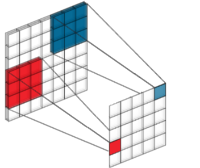
\includegraphics{img/faltung-klein.png}
	\captionof{figure}{Faltung eine 7x7x3 Matrix mit einem 3x3x3 Filter und erzeugter Aktivierungskarte \cite{knupp}}
	\label{img:faltung}
\end{minipage}

\subsubsection*{Verbindungsschicht}
Üblicherweise wird eine Verbindungsschicht zwischen zwei Faltungsschichten eingefügt. Seine Funktion besteht darin, schrittweise die Größe der Darstellung zu reduzieren, um die Anzahl der Parameter und dadurch die Berechnung des gesamten Netzwerkes zu verringern \cite{karpathy}. Sie ersetzt die Ausgabe eines Netzes an einem bestimmten Punkt durch eine statistische Zusammenfassung der naheliegendsten Ausgängen. Verschiedene Ansätze dafür sind Max Pooling, definiert nach Zhou \cite{zhou}, Übergabe der größte Zahl in einem rechteckigen Umfeld, Durchschnittsberechnung des Umfeldes oder ein gewichteter Durchschnitt basierend auf die Entfernung eines zentralen Punktes \cite{goodfellow}(355).

\subsubsection*{Vollständig verbundenen Schicht}
Neuronen in einer vollständig verbundenen Schicht haben Verbindungen zu allen Knoten der vorherigen Schicht. Ihre Aktivierung wird durch eine Matrixmultiplikation und einem Bias-Offset berechnet \cite{karpathy}. Die vollständig verbundenen Schicht wird als Ausgabeschicht verwendet um aus der Eingangsmatrix einen Vektor zu erzeugen.

\subsubsection*{Training}

\subsection{Vergleich verschiedener Ansätze}

\section{Experiment}

\subsection{Aufbau}

\subsection{Ergebnis}

\section{Vergleich mit Stand der Forschung und Ausblick}

%\bibliographystyle{abbrvdin}
\bibliographystyle{unsrt}
\bibliography{lit}

\end{multicols}

\end{document}
